\documentclass[a4paper,12pt]{article}
\usepackage[utf8]{inputenc}
\usepackage[spanish]{babel}
\usepackage{graphicx}
\usepackage{xcolor}
\usepackage{hyperref}
\usepackage[sorting=none]{biblatex}
\usepackage{float}
\addbibresource{bibliography/mybib.bib}
\usepackage{csquotes}
\graphicspath{{./images/}}
\hypersetup{colorlinks=true,linkcolor=blue,urlcolor=blue}
\begin{document}
\section{Problemática a resolver}
\paragraph{Detección de la enfermedad COVID-19 a través de una aplicación para dispositivos móviles.}
\section{Alcance del problema}
\paragraph{Creación de una aplicación para dispositivos móviles que permita, a través de completar un  cuestionario, registro sonoro del habla y tos, la ayuda en el diagnóstico de COVID-19.}
\section{Trasfondo}
\paragraph{La pandemia de gripe A (H1N1) de 2009-2010 fue una pandemia causada por la variante /09 del Influenzavirus A (subtipo H1N1). La enfermedad causada por esta nueva cepa viral es conocida como gripe porcina. El 30 de abril de 2009, la OMS decidió denominarla gripe A (H1N1).}
\paragraph{El origen de la infección es una variante de la cepa H1N1, con material genético proveniente de una cepa aviaria, dos cepas porcinas y una humana que sufrió una mutación y dio un salto entre especies (o heterocontagio) de los cerdos a los humanos, para después permitir el contagio de persona a persona.}
\paragraph{Los síntomas de este nuevo virus al lado de la influenza H1N1 en las personas son similares a los síntomas de la influenza o gripe estacional. Incluyen fiebre muy alta (38-40 ºC), tos seca recurrente, dolor de garganta, moqueo o secreción nasal, dolores en el cuerpo, dolor de cabeza, escalofríos, fatiga, dolor en los ojos, pérdida del apetito, problemas para respirar como falta de aliento. Una cantidad significativa de personas infectadas por este virus también informó tener vómito y diarrea.}
\paragraph{Entre enero de 2009 y septiembre de 2010, la cantidad de muertes a nivel mundial asciende a 19.000.
El 11 de marzo de 2020, la Organización Mundial de la Salud declaró oficialmente la pandemia de la nueva enfermedad SARS-CoV-2 (COVID-19).}
\paragraph{La enfermedad por coronavirus de 2019, más conocida como COVID-19, covid-19 o covid, e incorrectamente llamada neumonía por coronavirus, coronavirus o corona, es una enfermedad infecciosa causada por el SARS-CoV-2.}
\paragraph{Produce síntomas que incluyen fiebre, tos, disnea (dificultad respiratoria), mialgia (dolor muscular) y fatiga. En casos graves se caracteriza por producir neumonía, síndrome de dificultad respiratoria aguda, sepsis y choque circulatorio. Choque séptico es la forma más común en estos casos, pero los otros tipos también pueden ocurrir.}
\paragraph{Según la OMS, la infección es mortal entre el 0,5 \% y el 1 \% de los casos. No existe tratamiento específico; las medidas terapéuticas principales consisten en aliviar los síntomas y mantener las funciones vitales.}
\paragraph{Al mes de Abril de 2022 la cantidad de muertes producidas por la enfermedad COVID-19 asciende a las 6.100.000 personas a nivel mundial.}
\section{Propuesta}
\paragraph{Se sabe que una de las principales defensas con las que cuentan los Estados para combatirla es la rápida detección de los pacientes asintomáticos. Para que sea efectivo, se necesitan utilizar mecanismos que sean económicos, masivos y fácilmente escalables.}
\paragraph{Los médicos utilizan diariamente las señales de audio generadas por el cuerpo humano para el diagnóstico y seguimiento de enfermedades.}
\paragraph{A través de trabajos de investigación, se comienza a migrar con mayor ímpetu a tecnologías digitales para los exámenes clínicos con el objetivo de lograr su automatización a largo plazo.}
\paragraph{Estudios han probado que es posible generar un clasificador binario de aprendizaje automático simple que es capaz de segregar correctamente una persona asintomática COVID-19 de una sana basándose en registros de voz y tos de los pacientes.}
\paragraph{De esta manera, este trabajo busca ampliar el análisis automático de sonido en el diagnóstico de COVID-19, dando una metodología en la aplicación del análisis por inteligencia artificial en diagnósticos por análisis de sonido para esta y otras enfermedades actuales como así también enfermedades futuras que requieran una rápida respuesta colectiva.}
\section{Marco Teórico}
\subsection{Investigación del tema del problema (Legalidad, medicina, etc)}
\paragraph{La IA como herramienta: un marco para pensar la introducción de la Inteligencia Artificial en la provisión de servicios de salud.}
\paragraph{Así como la IA está cambiando la forma en que producimos, consumimos, trabajamos y nos comunicamos, también trajo consigo nuevas opciones para los gobiernos. Su incorporación en distintos ámbitos supone múltiples formas: desde la posibilidad de automatizar tareas, redistribuir responsabilidades entre humanos y máquinas, hasta facilitar el desarrollo de varias funciones basadas en el uso de datos (Deloitte Center for Government Insights, 2017).}
\paragraph{El sector de la salud es uno de los que más incorporó programas basados en inteligencia artificial, tanto desde el sector privado como el público. Inicialmente, su implementación se centró en el diagnóstico y detección de enfermedades. Un ejemplo de esto es el software DART, aplicado en Chile, que analiza imágenes oculares para el diagnóstico de retinopatía diabética. Según fuentes oficiales, esta herramienta permitiría triplicar la cantidad de estudios, al optimizar el uso de los recursos y volcar este ahorro hacia la adquisición de nuevos equipos y contratación de más personal médico y técnico, entre otras cosas (Ministerio de Salud de Chile, 2018). En línea con esto, otro caso es el del programa HeartFlow utilizado por la NHS en el Reino Unido para la creación modelos 3D del corazón y el flujo sanguíneo, permite detectar anomalías y proceder con el mejor tratamiento según el cuadro clínico.}
\paragraph{En la actualidad, los algoritmos también están colaborando en la definición e implementación de tratamientos. Si bien esta modalidad no se encuentra tan extendida como para los diagnósticos, múltiples investigaciones en curso resaltan su potencial. A modo de ejemplo, la Unión Europea está financiando una investigación de tres años en conjunto con organizaciones públicas y privadas de distintos países, para desarrollar un sistema llamado “PEPPER”, cuyo objetivo es dotar a los enfermos de diabetes de un dispositivo que - a través de IA - graduará dosis de insulina necesarias con alta precisión (Herrera, López y Martín, 2017).}
\paragraph{Además, la IA también está siendo utilizada para colaborar en la toma de decisiones en materia de salud pública, es decir, en programas gubernamentales como podrían ser políticas preventivas o programas de vacunación (Frenk, 1988). Este es el caso del hc1 Opioid Dashboard aplicado en Indiana (Estados Unidos), que utiliza técnicas de machine learning alimentada por resultados de laboratorio y bases de datos gubernamentales, con el fin de identificar niveles de uso de opioides a nivel barrial y enfocar las políticas preventivas en esos lugares.}
\paragraph{Si bien el sector público ha tenido un rol importante en la promoción y sostén de estos proyectos, ya sea garantizando el financiamiento de dichos programas o adoptando el uso de algoritmos para brindar servicios, el sector privado ha jugado un rol fundamental, ya que es allí donde estos desarrollos se producen a gran velocidad.}
\paragraph{En cuanto a sus efectos, distintos ejemplos resaltan las consecuencias positivas de aplicar la inteligencia artificial a los sistemas de salud. Las nuevas herramientas permitirían reemplazar viejos, lentos y costosos equipos y tratamientos, lo que a la larga racionaliza los sistemas de salud al volverlos más solventes y eficaces (Patel, 2018). Además, la inclusión de softwares inteligentes en las actividades médicas acelera la resolución de situaciones complejas, como la obstrucción de una arteria. Esto – a mayor escala – podría colaborar en la disminución de cuellos de botella existentes en los sistemas de salud públicos.}
\paragraph{Sin embargo, no todas las voces celebran el desembarco de la inteligencia artificial en la salud, y otras incluso cuestionan su efectividad. Tal es el caso de Watson for Oncology de IBM, un sistema utilizado en hospitales de más de 5 países para colaborar en el diagnóstico de pacientes con cáncer y en la definición sobre su atención clínica. Si bien este sistema está en modo beta (es decir, recién se puso a prueba), ya hubo varias denuncias alegando que el algoritmo utilizado derivó en una serie de recomendaciones de tratamientos “inseguros e incorrectos”, despertando de este modo dudas por la falta de validación clínica y de investigación revisada entre pares para corroborar su efectividad. Sin marcos de responsabilidad significativos, así como estructuras regulatorias sólidas, este tipo de experimentación sin control deriva en riesgos potenciales altos en materia de salud.}
\paragraph{Otras inquietudes refieren a la privacidad de los datos personales, una de las principales preocupaciones a la hora de regular a la IA. En concreto, y especialmente en un tema tan sensible como la salud, esto refiere a la importancia de contar con un consentimiento expreso e informado para el uso de estos datos y lo que distintos organismos puedan hacer con dicha información (e.g. Browne, 2018). Algunas estimaciones indican que, en Estados Unidos, solamente en el tercer trimestre de 2018, hubo 117 violaciones de datos de salud, derivando en la publicación de 4.4 millones de registros de pacientes.}
\paragraph{El presente trabajo busca ser un soporte complementario de calidad en el análisis de la enfermedad COVID-19 y no busca reemplazar el diagnóstico final de un profesional de la salud. Su objetivo es el de ser una herramienta más que agregue valor al juicio del profesional evaluador del caso.}
\subsection{Uso de datos personales y Habeas Data}
\paragraph{Con el objetivo de evitar incurrir en infracciones o cuestiones que competen al derecho de la normativa Argentina e Internacional, el software deberá indicar explícitamente en un contrato de usuario indicando específicamente que datos del usuario que utilice la aplicación se registrarán, que se conservará su anonimato en todo momento y que los datos que se persistirán en una bases de datos serán anónimos, con fines estadísticos y de aprendizaje automático para la inteligencia artificial y que no se guardará referencia de estos con el usuario.}
\paragraph{En la jurisprudencia argentina contamos con la acción de hábeas data que consta de una modalidad de amparo que permite a toda persona interesada acceder al conocimiento de los datos que consten en registros o bancos de datos públicos o privados destinados a proveer informes, y a exigir su supresión, rectificación, confidencialidad o actualización, en caso de falsedad o discriminación. Esta información debe referirse a cuestiones relacionadas con la intimidad y no puede ser utilizada por terceros sin el derecho reconocido a hacerlo.}
\subsection{Apoyo tecnológico}
\subsection{Recolección de Datos}
\paragraph{Para la recolección de datos, se utilizará un menú en la aplicación donde el usuario será guiado a través de una serie de sencillos pasos con la instrucción de cómo proceder a la vez que se le hará preguntas de su estado en general. Ya que posiblemente sea candidato a tener algún tipo de enfermedad respiratoria, se le mostrará formas seguras de hablar y toser sin poner en riesgo a su entorno, ni a sí mismo.}
\paragraph{Existe la posibilidad de que se generen muestras falsas, es decir, ruidos que no sean los solicitados por el sistema. Para ello, se puede crear un algoritmo de clasificación entrenado para detectar este tipo de muestras, excluyéndolas del análisis.}
\paragraph{Trabajos de investigación cuya hipótesis se basa en el análisis de muestras de audio desarrollan su estudio utilizando frameworks de aumento de gradiente extremo (eXtreme Gradient Boosting, XGBoost). Es una técnica de machine learning por regresión que permite crear un modelo de predicción por etapas.}
\paragraph{
\begin{figure}[H]
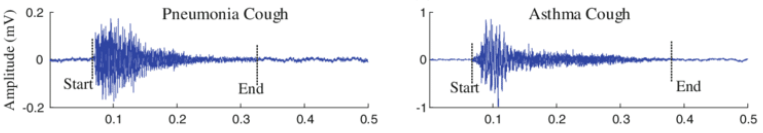
\includegraphics[width=\textwidth]{amplitude_pneumonia_asthma}
\end{figure}
\begin{figure}[H]
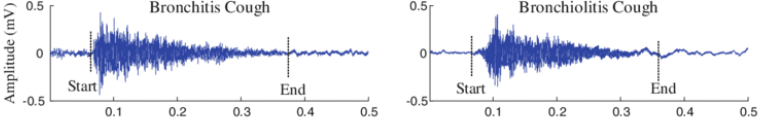
\includegraphics[width=\textwidth]{amplitude_bronchitis_bronchiolitis}
\end{figure}}
\paragraph{Usualmente, las muestras de audio se representan a lo largo de un periodo de tiempo en segundos y mostrando en el eje-y la amplitud de la onda, siendo esta una función de cambio en la presión alrededor del micrófono que capta el sonido.}
\paragraph{
\begin{figure}[H]
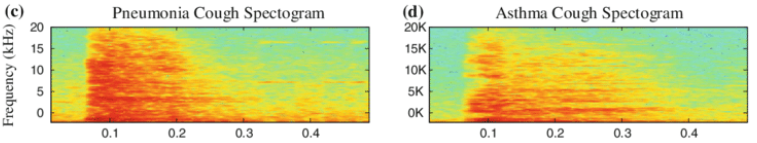
\includegraphics[width=\textwidth]{spectogram_pneumonia_asthma}
\end{figure}
\begin{figure}[H]
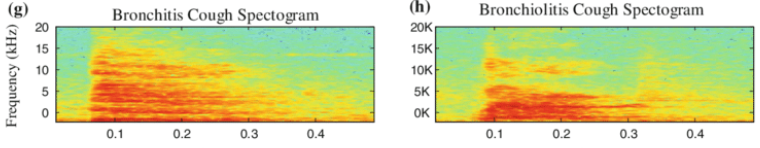
\includegraphics[width=\textwidth]{spectogram_bronchitis_bronchiolitis}
\end{figure}}
\paragraph{También se puede representar a través de un espectrograma, que es la representación visual del espectro de frecuencias de una señal que varía con el tiempo.}
\subsection{Demografía}
\paragraph{Se deberá analizar la localización geográfica proveniente de la muestra para compararla con estadísticas públicas y propias de la enfermedad. La misma servirá para acotar o descartar posibles diagnósticos según la procedencia y el comportamiento de la población para el caso de análisis.}
\paragraph{Para conseguir un nivel de fidelidad alto en el análisis de la información, es primordial obtener una amplia cantidad de muestras heterogéneas con la cual desarrollar la base de datos.}
\paragraph{Para el entrenamiento de la inteligencia artificial contamos con la base de datos pública provista por el Gobierno de la Ciudad de Buenos Aires la cual es de acceso público y que se pone a disposición para trabajos como el presente.}
\subsection{Estimación de la calidad del sonido}
\paragraph{Probablemente, cada usuario utilice un dispositivo diferente para grabar los audios de su tos y la voz. De la misma forma se tiene que considerar el sonido secundario como posible factor de interferencia (ruido) que puede presentarse al subir el archivo de audio ya que no todas las grabaciones estarán perfectamente aisladas.}
\paragraph{Para reducir el mismo se deberá contemplar un pre procesamiento de las muestras con el objetivo de su reducción sin afectar las partes de interés para su análisis.}
\subsection{Clasificación del Sonido}
\paragraph{Es importante tener una clasificación para los distintos tipos de voces y tos. La primera se puede agrupar los audios según el rango vocal, tesitura, puntos de transición vocal; mientras que la segunda puede discriminarse según la humedad, la duración, la frecuencia, la secades.}
\subsection{Procesamiento de datos}
\paragraph{
\begin{figure}[H]
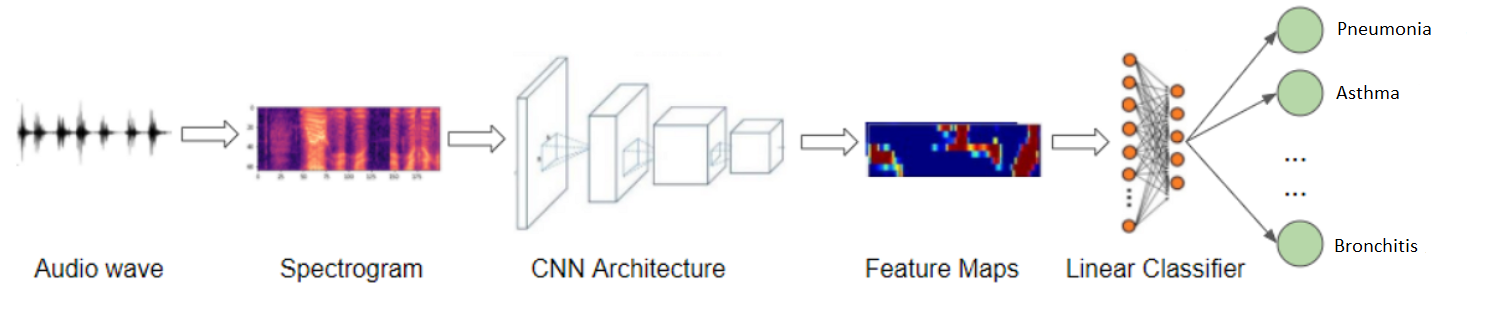
\includegraphics[width=\textwidth]{audiowave_to_classifier}
\end{figure}}
\paragraph{Para realizar el preprocesamiento del conjunto de datos, es necesario realizar una serie de pasos para extraer la información que le permita predecir la clase de muestra obtenida en un contexto de machine learning. Dicho proceso, buscará encontrar elementos distinguibles entre cada muestra.}
\paragraph{Por lo general, se recomienda extraer las ondas de audio generando Coeficientes Cepstrales en las Frecuencias de Mel o Mel Frequency Cepstral Coefficients. Se calculan al separar la señal en pequeños tramos, luego a cada uno se le aplica la transformada de Fourier discreta para obtener la potencia espectral de la señal. Al mismo se le aplica el banco de filtros correspondientes a la Escala Mel y se le suma las energías en cada uno.}
\paragraph{Por último, toma el logaritmo de todas las energías de cada frecuencia mel y se le aplica la transformada de coseno discreta.}
\paragraph{Existen frameworks como Librosa para ayudar con este tipo de trabajo.}
\subsection{Creación del Modelo}
\paragraph{Una vez obtenidos los espectrogramas, se puede utilizar una red neuronal convolucional de clasificación para procesar las imágenes. Frameworks como PyTorch trabajan con los bloques convolucionales que permiten generar los mapas de características para clasificar las muestras según las categorías predichas.}
\subsection{Aprendizaje}
\paragraph{Se definen las funciones para el optimizador, la pérdida y el programador para variar dinámicamente la tasa de aprendizaje a medida que avanza el entrenamiento.}
\paragraph{Se entrena el modelo en varios ciclos, procesando un lote de datos en cada iteración y se realiza un seguimiento de una métrica de precisión simple que mide el porcentaje de predicciones correctas.}
\subsection{Inferencia}
\paragraph{Se ejecuta un ciclo de inferencia teniendo cuidado de deshabilitar las actualizaciones de gradiente. El pase hacia adelante se ejecuta con el modelo para obtener predicciones, pero no necesitamos propagar hacia atrás ni ejecutar el optimizador.}
\section{Desarrollo}
\subsection{Requerimiento}
\paragraph{El propósito de este documento es construir un sistema en línea para la detección de la enfermedad COVID-19.
Este proyecto es un prototipo para el sistema de detección de la enfermedad COVID-19 y su uso está restringido dentro de la institución educativa. Se ha implementado bajo la guía de un profesor universitario.}
\paragraph{El sistema utilizará el archivo con audios de toses de personas grabadas por celular, segmentadas por COVID positivo y negativo según resultado de test RT-PCR provisto por la Secretaría de Innovación y Transformación Digital del Gobierno de la Ciudad de Buenos Aires\cite{dataset}.}
\paragraph{El análisis del procesamiento de sonido se logra a partir de la transformación de un archivo de audio a un espectrograma.\cite{espectrograma}}
\paragraph{El espectrograma se puede interpretar como una proyección en dos dimensiones de una sucesión de Transformación de Fourier\cite{fourier} de tramas consecutivas, donde la energía y el contenido frecuencial de la señal va variando a lo largo del tiempo.}
\paragraph{Para transformar una señal de audio en un espectrograma se utilizará la biblioteca de Python Librosa\cite{librosa}.}
\paragraph{Utilizaremos el framework FFmpeg\cite{ffmpeg} para convertir los archivos de audios de ogg a wav para poder procesarlos correctamente con Librosa.}
\subsection{Diseño de la Solución}
\paragraph{Diseño realizado en: \href{https://www.figma.com/proto/M8RWGFdiOidZSZONJyYMPn/TFG?node-id=2\%3A3&starting-point-node-id=2\%3A3}{Figma.}}
\subsection{Arquitectura del Producto}
\paragraph{
\begin{figure}[H]
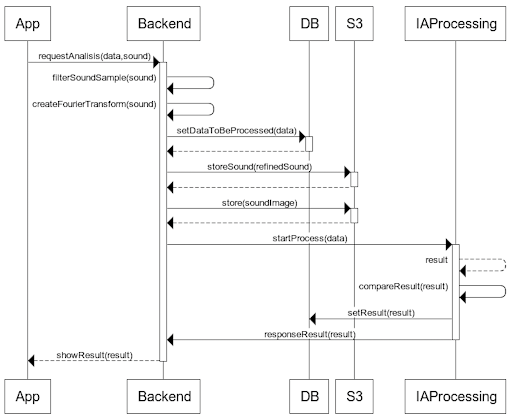
\includegraphics[width=\textwidth]{diagrama_de_secuencia}
\end{figure}}
\subsection{Tecnologías}
\subsection{Proof of Concept}
\section{Conclusión}
\printbibliography
\end{document}